\section{Introduction to the Problem}

The objective of this project is to study the flow around the surfaces of a glider airplane composed by a wing, a canard and a vertical tail plane, all attached thanks to a thin, negligible, rigid rod, as shown in Figure \ref{fig:GliderConfig}. Both wing and canard have zero sweep angle and a trapezoidal shape, with their geometries defined by the following values:

\[b = 24 m;     cr = 1.8 m;     ct = 1.2 m\]
\[b_h = 6 m;     cr_h = 1 m;     ct_h = 0.6 m\]

The airfoils employed are the NACA 22112 and NACA 0012 for the wing and canard respectively. Incidence angles are $0^\circ$ for the wing and $3^\circ$ for the canard.

\begin{figure}[H]
    \centering
    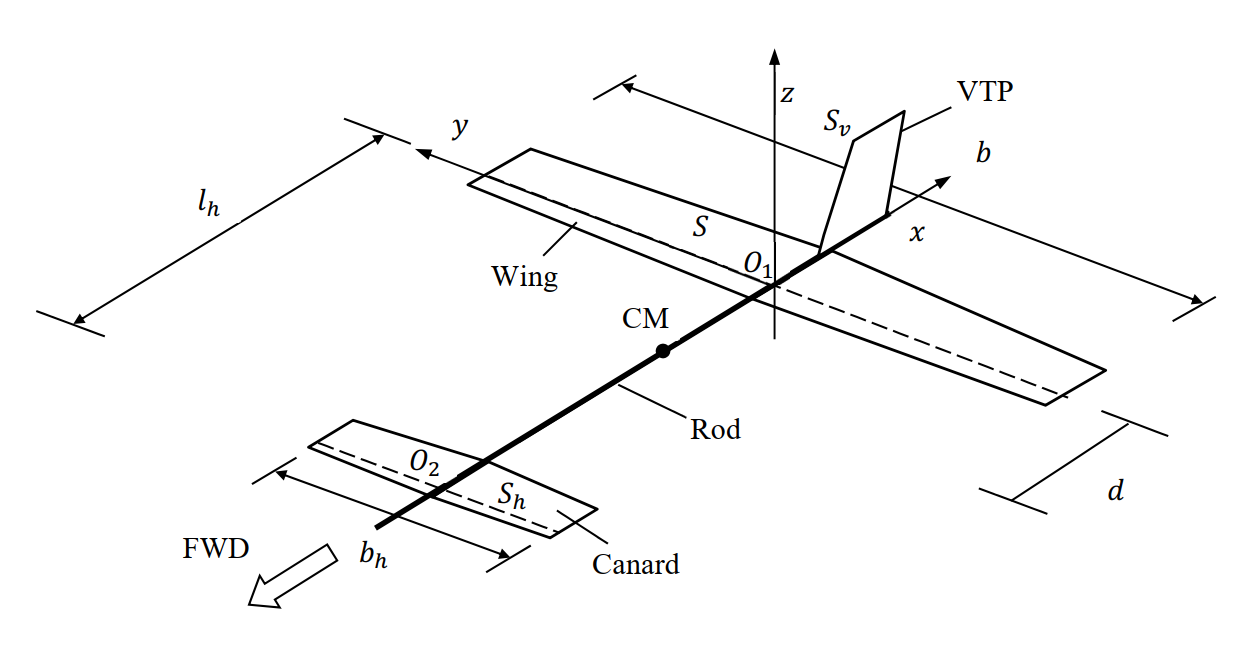
\includegraphics[width=0.8\linewidth]{imatges/gliderconfig.png}
    \caption{Configuration of the studied glider aircraft.}
    \label{fig:GliderConfig}
\end{figure}

The problem is divided into the following parts:
\begin{itemize}
    \item \textbf{Part 1:} Implementation of the constant strength vortex method. This part is itself divided in two, firstly the wing is studied with the objective to compute relevant aerodynamic coefficients, then the flow around the canard is calculated, considering it a combination of two airfoils, in order to understand the aerodynamic effects of having two areodynamic components very close together as can be observed in Figure \ref{fig:CanardConfig}.
    
    \begin{figure}[H]
        \centering
        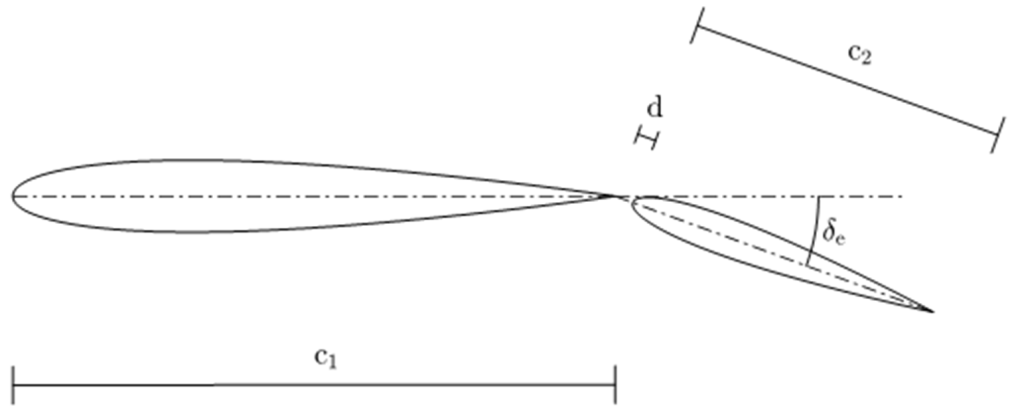
\includegraphics[width=0.4\linewidth]{imatges/canardconfig.png}
        \caption{Configuration of the canard, with two NACA 0012 in succession.}
        \label{fig:CanardConfig}
    \end{figure}
    
    \item \textbf{Part 2:} Implementation of Prandtl's lifting line model.

\end{itemize}
